\chapter{Introducción}
El osciloscopio de la marca Tektronix, específicamente el modelo TDS 360 permite una comunicación serial utilizando el puerto RS232. Actualmente existen adaptadores de RS232 a USB con lo cual se diseño una aplicación haciendo uso del Software App Designer (de la suite de MatLab) que logre iniciar la comunicación, configurar el osciloscopio y recibir el vector de valores correspondientes a las muestras almacenadas en el registro del Osciloscopio.

\section{Instalación del Driver Prolific}
Dado que Windows instala una versión del driver que no permite hacer uso del adaptador (ya que reconoce que el chip no es original), se deberá instalar el Driver adecuado. Para eso, en la seccion de \textbf{Administrador de Dispositivos}, se debe desinstalar completamente el que instala Windows:

\vspace{5mm}

\begin{center}
	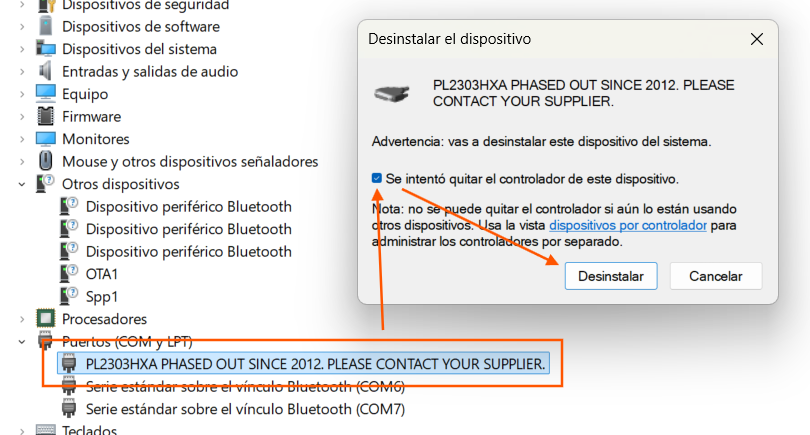
\includegraphics[width=0.8\columnwidth]{images/Driver_01.png}
	\captionsetup{type=figure}
	\caption{Adm. de Dispositivos - Eliminar Driver}
	\label{fig:eliminar-driver}
\end{center}

Luego de este paso, \underline{sin desconectar el adaptador}, se procede a instalar el nuevo driver usando el instalador adjunto al instructivo.

En este punto, si la instalación fue correcta, entonces se utiliza la opción del menú: \textbf{Buscar cambios de Hardware}. En la lista deberá aparecer el nombre:

\begin{center}
	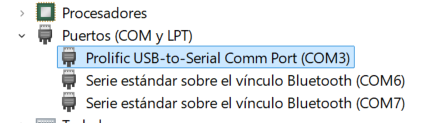
\includegraphics[width=0.45\columnwidth]{images/Driver_02.png}
	\captionsetup{type=figure}
	\caption{Adm. de Dispositivos - Driver Prolific}
	\label{fig:listado-driver-ok}
\end{center}

Si luego de refrescar la lista, sigue apareciendo el driver anterior, se podrá forzar la actualización de la siguiente forma:

\vfill
\newpage

\begin{enumerate}
	\item Seleccionar el elemento de la lista y en las opciones desplegables elegir \textit{Actualizar controlador}.
	\item Seleccionar \textit{Examinar mi PC en busca de controladores}.
	\item Seleccionar \textit{Elegir en una lista de controladores disponibles en el equipo}.
	\item Y de la lista, seleccionar \textbf{Prolific USB-to-Serial Comm Port}
\end{enumerate}

\vspace{5mm}

\textit{\textbf{Nota:} La instalación automatica del driver por parte de Windows se logra porque Windows Update está habilitado. En caso de requerir desactivar esta funcionalidad momentaneamente se puede usar el ejecutable \href{https://www.sordum.org/9470/windows-update-blocker-v1-8/}{\underline{Windows Update Blocker v1.8}})}



\section{Requisitos de la Aplicación}
La primera versión que se logro realizar, tiene el siguiente aspecto.
\begin{center}
	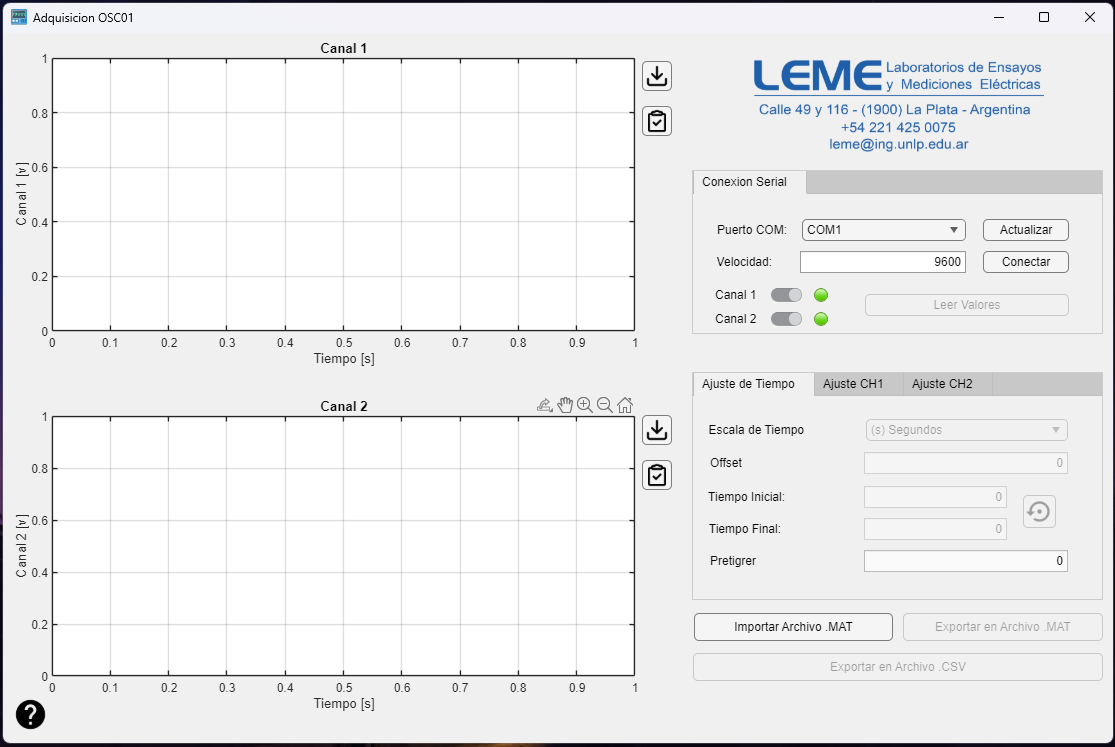
\includegraphics[width=0.8\columnwidth]{images/version_preliminar.png}
	\captionsetup{type=figure}
	\caption{Versión preliminar - Diseño}
	\label{fig:app-pantalla-principal}
\end{center}
El diseño es sencillo, se intenta que disponga de las siguientes funcionalidades:

\begin{itemize}
	\item Que permita configurar los valores esenciales de la comunicación serial, por ejemplo, el puerto \textbf{COM} y los \textbf{Bits por segundo}.
	\item Que verifique la correcta comunicación con el Osciloscopio.
	\item Que luego de solicitar los valores, se disponga de casilleros donde se pueda ajustar los limites de tiempo.
	\item Que los limites del eje vertical de cada canal se pueda modificar.
	\item Que se permita modificar los títulos y las leyendas de cada gráfica.
	\item Que cada canal, disponga de un casillero donde se pueda ingresar un factor, con el fin de aplicar tal valor a cada valor del eje vertical.
\end{itemize}




\section{Comunicación Serial}
En primer lugar, al usar un conversor de RS232 a USB, se procedió a enviar los primeros comandos usando el \textbf{Monitor Serial} del Arduino IDE (Disponible en el \href{https://www.arduino.cc/en/software}{\underline{Link}}).
Los comandos que se usan son los que se enumeran a continuacion. En aquellos donde se especifique \code{CHn}, podra valer \code{CH1} o \code{CH2}.

\begin{itemize}
	\item \code{DATA:ENCDG ASCII}: Configura la codificación de los valores que recibo cuando solicito las muestras almacenadas.
	Esta codificación podrá ser: \code{ASCII}, \code{RIbynary}
	\item \code{HEADER OFF}: Permite que las respuestas no contengan el identificador del comando, de esta forma la respuesta sera unicamente los valores que solicitemos.
	\item \code{DATA:WIDTH 2}: Al configurar en \code{2}, cuando se soliciten las muestras tomadas, el osciloscopio nos devolverá los valores con usando 2 bytes.
	\item \code{DATA:SOURCE CHn}: Permite seleccionar un canal especifico, para luego descargar los valores de este canal.
	\item \code{HORIZONTAL:Main?}: El osciloscopio devolverá el valor de los $^s/_{div}$
	\item \code{CHn:SCALE?}: Permite obtener el valor de los $^v/_{div}$. La elección del canal se hace con \code{CH1} o \code{CH2}.
	\item \code{WFMPRE:CHn:XINCR?}: Permite obtener el valor del tiempo entre dos muestras consecutivas.
	\item \code{WFMPRE:CHn:YMULT?}: Permite obtener el valor por el cual se debe multiplicar cada muestra.
	\item \code{WFMPRE:CHn:YZERO?}: Devuelve el valor del offset vertical.
	\item \code{WFMPRE:CHn:YOFF?}: Devuelve el valor del offset de voltage.
	\item \code{CURVE?}: Al enviar este comando, el osciloscopio devolvera los puntos guardados en su registro, en el formato especificado por \code{DATA:ENCDG}.
	\item \code{HORIZONTAL:TRIGGER:POSITION?}: Es el valor, en porcentaje, de tiempo con respecto a la ventana total de tiempo que se tiene como pre-triger.
\end{itemize}

\vspace{5mm}
El procedimiento para obtener el vector del canal 1 es el siguiente:


\begin{lstlisting}[style=rawStyle]
write("DATA:ENCDG RIBINARY");
write("HEADER OFF);
write("DATA:WIDTH 2");

write("DATA:SOURCE CH1");
write("CURVE?");

xincr = writeread("WFMPRE:CH1:XINCR?");
ymult = writeread("WFMPRE:CH1:YMULT?");
yzero = writeread("WFMPRE:CH1:YZERO?");
yoff  = writeread("WFMPRE:CH1:YOFF?");

adc_raw = readbinblock();
\end{lstlisting}

Finalmente, una vez que se logre recibir el vector de puntos, y los demás valores se procede con la conversión de unidades, con el objetivo de armar los vectores de tiempo y tensión.

\begin{equation}
	volts \;=\; (adc\_raw - y_{off}) \cdot y_{mult} + y_{zero}
	\label{eq:001}
\end{equation}
\begin{equation}
	t \;=\; 0 \;:\; x_{incr} \;:\; (length(volts) - 1) \cdot x_{incr} 
	\label{eq:002}
\end{equation}

La ecuación \ref{eq:002} hace uso de la sintaxis de Matlab, logrando formar un vector desde cero hasta la ultima muestra leida, con un tiempo entre muestra de $x_{incr}$.

Estos comandos fueron los necesarios para descargar todos los valores y datos del canal 1, para hacer uso del canal 2, se repite desde la linea 4 (\texttt{write("DATA:SOURCE CH1);}) haciendo uso del \texttt{CH2}.




